% Options for packages loaded elsewhere
\PassOptionsToPackage{unicode}{hyperref}
\PassOptionsToPackage{hyphens}{url}
\PassOptionsToPackage{dvipsnames,svgnames,x11names}{xcolor}
%
\documentclass[
]{article}
\usepackage{amsmath,amssymb}
\usepackage{iftex}
\ifPDFTeX
  \usepackage[T1]{fontenc}
  \usepackage[utf8]{inputenc}
  \usepackage{textcomp} % provide euro and other symbols
\else % if luatex or xetex
  \usepackage{unicode-math} % this also loads fontspec
  \defaultfontfeatures{Scale=MatchLowercase}
  \defaultfontfeatures[\rmfamily]{Ligatures=TeX,Scale=1}
\fi
\usepackage{lmodern}
\ifPDFTeX\else
  % xetex/luatex font selection
\fi
% Use upquote if available, for straight quotes in verbatim environments
\IfFileExists{upquote.sty}{\usepackage{upquote}}{}
\IfFileExists{microtype.sty}{% use microtype if available
  \usepackage[]{microtype}
  \UseMicrotypeSet[protrusion]{basicmath} % disable protrusion for tt fonts
}{}
\makeatletter
\@ifundefined{KOMAClassName}{% if non-KOMA class
  \IfFileExists{parskip.sty}{%
    \usepackage{parskip}
  }{% else
    \setlength{\parindent}{0pt}
    \setlength{\parskip}{6pt plus 2pt minus 1pt}}
}{% if KOMA class
  \KOMAoptions{parskip=half}}
\makeatother
\usepackage{xcolor}
\usepackage[margin=1in]{geometry}
\usepackage{longtable,booktabs,array}
\usepackage{calc} % for calculating minipage widths
% Correct order of tables after \paragraph or \subparagraph
\usepackage{etoolbox}
\makeatletter
\patchcmd\longtable{\par}{\if@noskipsec\mbox{}\fi\par}{}{}
\makeatother
% Allow footnotes in longtable head/foot
\IfFileExists{footnotehyper.sty}{\usepackage{footnotehyper}}{\usepackage{footnote}}
\makesavenoteenv{longtable}
\usepackage{graphicx}
\makeatletter
\def\maxwidth{\ifdim\Gin@nat@width>\linewidth\linewidth\else\Gin@nat@width\fi}
\def\maxheight{\ifdim\Gin@nat@height>\textheight\textheight\else\Gin@nat@height\fi}
\makeatother
% Scale images if necessary, so that they will not overflow the page
% margins by default, and it is still possible to overwrite the defaults
% using explicit options in \includegraphics[width, height, ...]{}
\setkeys{Gin}{width=\maxwidth,height=\maxheight,keepaspectratio}
% Set default figure placement to htbp
\makeatletter
\def\fps@figure{htbp}
\makeatother
\setlength{\emergencystretch}{3em} % prevent overfull lines
\providecommand{\tightlist}{%
  \setlength{\itemsep}{0pt}\setlength{\parskip}{0pt}}
\setcounter{secnumdepth}{5}
\ifLuaTeX
\usepackage[bidi=basic]{babel}
\else
\usepackage[bidi=default]{babel}
\fi
\babelprovide[main,import]{french}
% get rid of language-specific shorthands (see #6817):
\let\LanguageShortHands\languageshorthands
\def\languageshorthands#1{}
\usepackage{amsmath} \usepackage{geometry} \usepackage{pdfpages} \usepackage{fontspec} \usepackage{pdfpages} \usepackage{graphicx} \usepackage{amsmath} \usepackage{atbegshi} \usepackage{fancyhdr} \usepackage{tocloft} \usepackage{tcolorbox} \usepackage{xcolor} \definecolor{bleu}{RGB}{0,0,255} \usepackage{everypage} \usepackage{everypage} \usepackage{graphicx} \usepackage{fancyhdr} \pagestyle{fancy} \definecolor{mybrown}{RGB}{139,69,19} \fancyhead[R]{}
\ifLuaTeX
  \usepackage{selnolig}  % disable illegal ligatures
\fi
\IfFileExists{bookmark.sty}{\usepackage{bookmark}}{\usepackage{hyperref}}
\IfFileExists{xurl.sty}{\usepackage{xurl}}{} % add URL line breaks if available
\urlstyle{same}
\hypersetup{
  pdflang={fr},
  colorlinks=true,
  linkcolor={Maroon},
  filecolor={Maroon},
  citecolor={Blue},
  urlcolor={blue},
  pdfcreator={LaTeX via pandoc}}

\author{}
\date{\vspace{-2.5em}}

\begin{document}

\setcounter{tocdepth}{5}                
\renewcommand\contentsname{\begin{center}\textcolor{brown}{Sommaire}\end{center}}

\AtBeginShipout{
  \ifnum\value{page}=1\thispagestyle{empty}\fi}

\pagestyle{fancy}
\fancyhf{}
\renewcommand{\headrulewidth}{0.4pt}
\renewcommand{\footrulewidth}{0.4pt}
\fancyhead[L]{Elèves Ingénieurs}
\fancyhead[R]{\textcolor{brown}{@Alex, Ali, Richard \& Toussaint}}
\fancyfoot[C]{\thepage}
\fancyfoot[L]{Mars 2025}
\fancyfoot[R]{Projet Statistique}

\AddEverypageHook{
  \ifnum\value{page}>1 
    \fancyhead[L]{Elèves Ingénieurs}
    \fancyhead[R]{\textcolor{brown}{@Alex, Ali, Richard \& Toussaint}}
    \fancyfoot[C]{\thepage}
    \fancyfoot[L]{Mars 2025}
    \fancyfoot[R]{Projet Statistique}
  \else
    \fancyhead[L]{} 
    \fancyhead[R]{}
    \fancyfoot[C]{}
    \fancyfoot[R]{}
  \fi
}

\tableofcontents

\newpage

\renewcommand\listtablename{\begin{center}\textcolor{brown}{Liste des Tableaux}\end{center}}
\renewcommand\listfigurename{\begin{center}\textcolor{brown}{Liste des Figures}\end{center}} 

\setlength{\cftfignumwidth}{3em}
\setlength{\cfttabnumwidth}{3em}

\listoftables

\newpage

\listoffigures

\newpage

\hypertarget{introduction}{%
\section{Introduction}\label{introduction}}

\hypertarget{pruxe9sentation-du-contexte}{%
\section{Présentation du contexte}\label{pruxe9sentation-du-contexte}}

\hypertarget{intuxe9ruxeat-de-luxe9tude}{%
\subsection{Intérêt de l'étude}\label{intuxe9ruxeat-de-luxe9tude}}

\hypertarget{cadre-conceptuel-de-luxe9tude}{%
\subsection{Cadre conceptuel de
l'étude}\label{cadre-conceptuel-de-luxe9tude}}

\hypertarget{pruxe9sentation-des-donnuxe9es}{%
\subsection{Présentation des
données}\label{pruxe9sentation-des-donnuxe9es}}

Les données que nous avons utilisées nous proviennent de \ldots{}

\hypertarget{muxe9thodologie}{%
\section{Méthodologie}\label{muxe9thodologie}}

\hypertarget{motivation}{%
\subsection{Motivation}\label{motivation}}

Les modèles linéaires généralisés à effets mixtes (GLMM) combinent :

\begin{itemize}
\item
  Les caractéristiques des modèles linéaires généralisés (GLM) pour
  modéliser des variables non-normalement distribuées.
\item
  Les propriétés des modèles à effets mixtes pour gérer des données
  groupées ou hiérarchiques.
\end{itemize}

\hypertarget{moduxe8les-linuxe9aires-guxe9nuxe9ralisuxe9s}{%
\subsection{Modèles Linéaires
Généralisés}\label{moduxe8les-linuxe9aires-guxe9nuxe9ralisuxe9s}}

Un GLM relie le prédicteur linéaire \(\eta\) à la moyenne \(\mu\) de la
réponse à travers une fonction de lien \(g\) :\\
\[ g(\mu) = \eta = \beta_0 + \sum_{i=1}^m \beta_i x_i \]\\
Les distributions possibles incluent :

\begin{itemize}
\item
  \textbf{Normale} : Régression linéaire classique, avec lien identité.
\item
  \textbf{Binomiale} : Régression logistique pour données binaires, avec
  lien logit.
\item
  \textbf{Poisson} : Régression de Poisson pour données de comptage,
  avec lien logarithmique.
\end{itemize}

\hypertarget{ruxe9gression-logistique}{%
\subsubsection{Régression Logistique}\label{ruxe9gression-logistique}}

Modélise une réponse binaire (\(y \sim B(n, p)\)), où \(p\) est la
probabilité de succès :\\
\[ P(y | n, p) = \binom{n}{y} p^y (1-p)^{n-y} \]\\
La probabilité \(p\) est reliée au prédicteur par la fonction logistique
:\\
\[ p = \frac{1}{1 + e^{-\eta}} \quad \text{où} \quad \eta = \beta_0 + \sum_{i=1}^m \beta_i x_i. \]\\
Le log-vraisemblance est exprimé comme :\\
\[ \ell(\boldsymbol{\beta}) = \sum_{i=1}^n \left[ y_i \log{p_i} + (1-y_i) \log{(1-p_i)} \right]. \]

\hypertarget{ruxe9gression-de-poisson}{%
\subsubsection{Régression de Poisson}\label{ruxe9gression-de-poisson}}

Utilisée pour modéliser des données de comptage
(\(y \sim Pois(\lambda)\)), où \(\lambda\) est la moyenne et la variance
:\\
\[ P(y | \lambda) = \frac{\lambda^y}{y!} e^{-\lambda} \]\\
Le lien logarithmique assure \(\lambda > 0\) :\\
\[ \log{\lambda} = \beta_0 + \sum_{i=1}^m \beta_i x_i \]\\
L'espérance est \(E[y] = \lambda\).

\hypertarget{moduxe8les-linuxe9aires-mixtes}{%
\subsection{Modèles Linéaires
Mixtes}\label{moduxe8les-linuxe9aires-mixtes}}

Ces modèles ajoutent des termes d'effets aléatoires
\(\mathbf{Z} \mathbf{u}\) au prédicteur linéaire :\\
\[ \mathbf{y} = \mathbf{X} \boldsymbol{\beta} + \mathbf{Z} \mathbf{u} + \boldsymbol{\varepsilon}, \]\\
avec :

\begin{itemize}
\item
  \(\mathbf{u} \sim N(\mathbf{0}, \mathbf{G})\), les effets aléatoires.
\item
  \(\boldsymbol{\varepsilon} \sim N(\mathbf{0}, \mathbf{R})\), les
  résidus.
\end{itemize}

La matrice de covariance totale est :\\
\[ \mathrm{Var}(\mathbf{y}) = \mathbf{Z} \mathbf{G} \mathbf{Z}^T + \mathbf{R}. \]\\
Les paramètres sont estimés par maximum de vraisemblance (ML) ou par
vraisemblance restreinte (REML).

\hypertarget{moduxe8les-linuxe9aires-guxe9nuxe9ralisuxe9s-uxe0-effets-mixtes-glmm}{%
\subsection{Modèles Linéaires Généralisés à Effets Mixtes
(GLMM)}\label{moduxe8les-linuxe9aires-guxe9nuxe9ralisuxe9s-uxe0-effets-mixtes-glmm}}

Un GLMM étend les GLM en intégrant des effets aléatoires :\\
\[ g(\mu) = \mathbf{X} \boldsymbol{\beta} + \mathbf{Z} \mathbf{u}, \]\\
où :\\
- \(g(\cdot)\) est la fonction de lien.\\
- \(\mathbf{u} \sim N(\mathbf{0}, \mathbf{G})\) est le vecteur d'effets
aléatoires.

Les paramètres sont estimés via des méthodes comme :\\
- Approximations Laplaciennes.\\
- Quadrature gaussienne adaptative.\\
- Méthodes MCMC (chaînes de Markov Monte Carlo).

\hypertarget{pruxe9dictions-et-simulations}{%
\subsection{Prédictions et
Simulations}\label{pruxe9dictions-et-simulations}}

Les GLMM permettent deux types de prédictions :\\
- \textbf{Conditionnelles} : Basées sur les effets aléatoires
spécifiques (\(\mathbf{u}\)).\\
- \textbf{Marginales} : En intégrant sur les effets aléatoires.

Les simulations utilisent des approches paramétriques pour évaluer la
variabilité et tester les hypothèses. Une approche courante est le
bootstrap paramétrique :\\
1. Générer des données simulées basées sur les paramètres estimés.\\
2. Réajuster le modèle pour chaque jeu de données simulé.\\
3. Analyser la distribution des estimations obtenues.

\hypertarget{analyse-des-ruxe9sultats}{%
\section{Analyse des résultats}\label{analyse-des-ruxe9sultats}}

\hypertarget{analyse-descriptive}{%
\subsection{Analyse descriptive}\label{analyse-descriptive}}

Dans cette partie, nous allons réaliser quelques statistiques
descriptives sur nos données.

\hypertarget{analyse-univariuxe9e}{%
\subsubsection{Analyse univariée}\label{analyse-univariuxe9e}}

\begin{verbatim}
##    Min. 1st Qu.  Median    Mean 3rd Qu.    Max. 
##    1037    5993    9127   19130   17290  765833
\end{verbatim}

L'analyse des statistiques descriptives sur le nombre de consultations
annuelles de médecin généraliste entre 2018 et 2022 révèle une
distribution fortement asymétrique à droite, avec une grande dispersion
des données. La moyenne de 19130 consultations, nettement supérieure à
la médiane de 9127, indique la présence de valeurs extrêmes tirant la
distribution vers le haut. Cette asymétrie est confirmée par l'écart
considérable entre le minimum de 1037 et le maximum de 765833
consultations par an.

La moitié des médecins généralistes effectuent entre 5993 et 17290
consultations annuellement, ce qui suggère une variabilité importante
dans la charge de travail. La médiane de 9127 consultations par an,
équivalant à environ 25 consultations par jour ouvrable, semble plus
représentative de l'activité typique d'un médecin généraliste que la
moyenne influencée par les valeurs extrêmes. Ces statistiques mettent en
lumière la diversité des pratiques et des charges de travail parmi les
médecins généralistes, avec potentiellement quelques cas atypiques
présentant un volume de consultations exceptionnellement élevé.

Le nombre de visites pouvant potentiellement être influencé par la
taille de la commune et donc par sa population, nous avons éliminer cet
effet en calculant le taux de consultations qui n'est autre que le
nombre de consultations moyennes par personnes.

\begin{figure}

{\centering 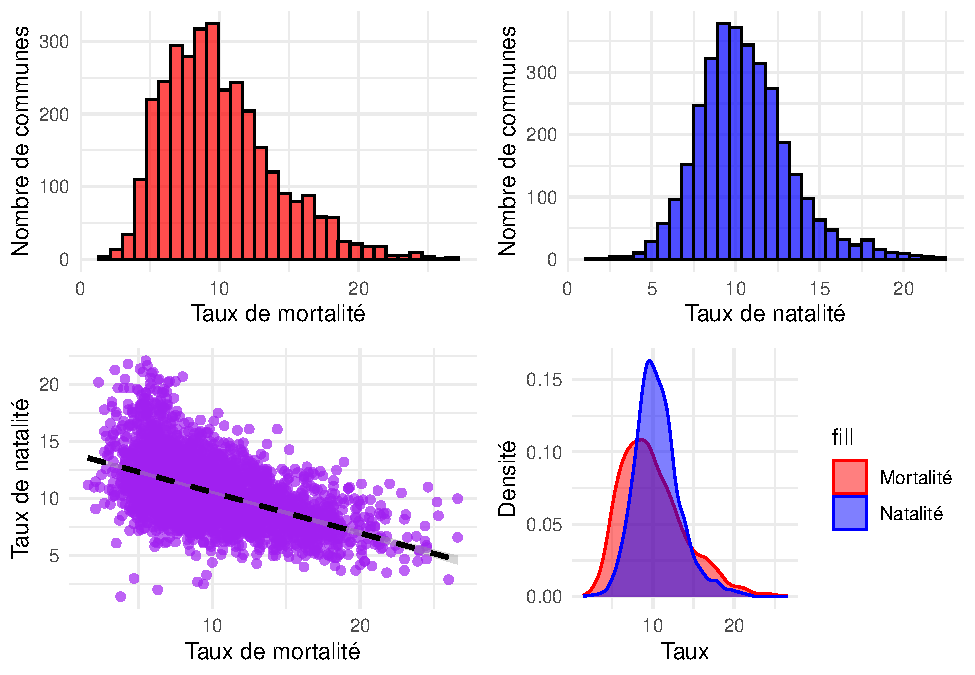
\includegraphics{Rapport_Projet_Stat_Ensai_files/figure-latex/unnamed-chunk-4-1} 

}

\caption{Répartition du nombre et du taux de consultations}\label{fig:unnamed-chunk-4}
\end{figure}

\hypertarget{analyse-bivariuxe9e}{%
\subsubsection{Analyse bivariée}\label{analyse-bivariuxe9e}}

Nous allons ici, voir s'il y a un lien à priori entre le taux de
consultation et certaines de nos variables explicatives. Ainsi, nous
avons d'abord réalisé une analyse descriptive bivariée puis nous avons
calculé la corrélation de Pearson pour évaluer le lien linéaire entre le
taux de consulation et des variables telles que la population totale, la
part des personnes agées (75 ans et plus), la part de quelques CSP
(ouvriers et retraités).

\hypertarget{taux-de-consultation-et-population-totale}{%
\paragraph{Taux de consultation et population
totale}\label{taux-de-consultation-et-population-totale}}

\begin{longtable}[]{@{}lr@{}}
\caption{Taux de consultations selon la taille de la
commune}\tabularnewline
\toprule\noalign{}
taille\_commune & Taux de consulations \\
\midrule\noalign{}
\endfirsthead
\toprule\noalign{}
taille\_commune & Taux de consulations \\
\midrule\noalign{}
\endhead
\bottomrule\noalign{}
\endlastfoot
Grande (\textgreater{} 8974) & 1.526810 \\
Moyenne (4849 - 8974) & 1.456356 \\
Petite (\textless= 4848) & 1.383861 \\
\end{longtable}

En divisant les communes en trois groupes égaux (ou presque égaux) en
fonction de la population totale, il ressort qu'en moyenne, plus la
taille de la commune est importante plus le taux de consulations est
élevé.

\hypertarget{taux-de-consultation-et-population-uxe2guxe9e}{%
\paragraph{Taux de consultation et population
âgée}\label{taux-de-consultation-et-population-uxe2guxe9e}}

\begin{longtable}[]{@{}lr@{}}
\caption{Taux de consultations selon la population âgée}\tabularnewline
\toprule\noalign{}
population\_agee\_importante & consultations\_moyennes \\
\midrule\noalign{}
\endfirsthead
\toprule\noalign{}
population\_agee\_importante & consultations\_moyennes \\
\midrule\noalign{}
\endhead
\bottomrule\noalign{}
\endlastfoot
Non (\textless= 670) & 1.501111 \\
Oui (\textgreater{} 670) & 1.410213 \\
\end{longtable}

\begin{figure}

{\centering 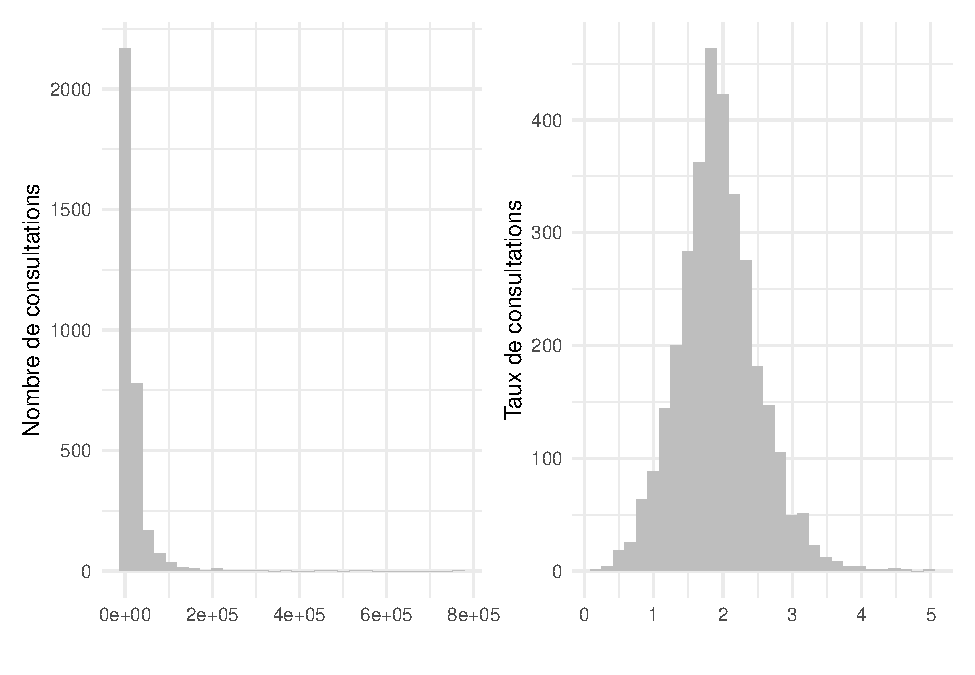
\includegraphics{Rapport_Projet_Stat_Ensai_files/figure-latex/unnamed-chunk-7-1} 

}

\caption{Relation entre taux de consultations et part des plus de 75 ans}\label{fig:unnamed-chunk-7}
\end{figure}

Les communes avec une population âgée importante (communes dont la
population âgée de 75 ans ou plus est supérieure à la médiane) ont en
moyenne un taux de consultations plus faible.

\hypertarget{taux-de-consultation-et-csp}{%
\paragraph{Taux de consultation et
CSP}\label{taux-de-consultation-et-csp}}

\begin{figure}

{\centering 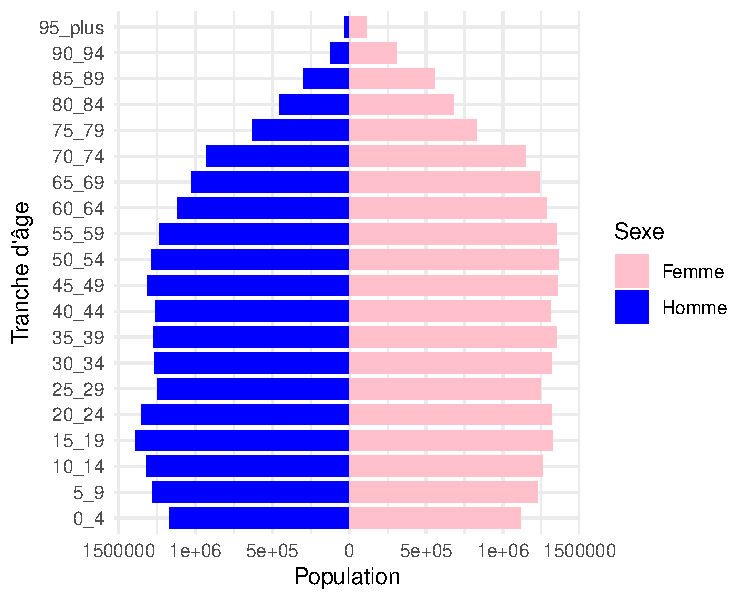
\includegraphics{Rapport_Projet_Stat_Ensai_files/figure-latex/unnamed-chunk-8-1} 

}

\caption{Relations entre le taux de consultatiosn et certaines le nombre de certaines catégories socioprofessionnelle}\label{fig:unnamed-chunk-8}
\end{figure}

Aucune catégorie ne semble montrer une relation linéaire évidente avec
le taux de visite. Par ailleurs, pour toutes les catégories
socio-professionnelles, la majorité des communes se situent dans une
plage de proportions faibles, ce qui limite la variabilité observable
dans les relations. Une analyse statistique supplémentaire, comme le
calcul de corrélations, serait nécessaire pour confirmer ou infirmer les
relations observées visuellement.

\hypertarget{analyse-de-corruxe9lation}{%
\paragraph{Analyse de corrélation}\label{analyse-de-corruxe9lation}}

Les résultats de la corrélation de Pearson sont consignées dans le
tableau suivant :

\begin{longtable}[]{@{}
  >{\raggedright\arraybackslash}p{(\columnwidth - 8\tabcolsep) * \real{0.0543}}
  >{\raggedright\arraybackslash}p{(\columnwidth - 8\tabcolsep) * \real{0.5652}}
  >{\raggedleft\arraybackslash}p{(\columnwidth - 8\tabcolsep) * \real{0.1304}}
  >{\raggedleft\arraybackslash}p{(\columnwidth - 8\tabcolsep) * \real{0.1087}}
  >{\raggedright\arraybackslash}p{(\columnwidth - 8\tabcolsep) * \real{0.1413}}@{}}
\caption{Corrélations de Pearson entre le taux de consultation et les
autres variables}\tabularnewline
\toprule\noalign{}
\begin{minipage}[b]{\linewidth}\raggedright
\end{minipage} & \begin{minipage}[b]{\linewidth}\raggedright
Variable
\end{minipage} & \begin{minipage}[b]{\linewidth}\raggedleft
Correlation
\end{minipage} & \begin{minipage}[b]{\linewidth}\raggedleft
P\_value
\end{minipage} & \begin{minipage}[b]{\linewidth}\raggedright
Significatif
\end{minipage} \\
\midrule\noalign{}
\endfirsthead
\toprule\noalign{}
\begin{minipage}[b]{\linewidth}\raggedright
\end{minipage} & \begin{minipage}[b]{\linewidth}\raggedright
Variable
\end{minipage} & \begin{minipage}[b]{\linewidth}\raggedleft
Correlation
\end{minipage} & \begin{minipage}[b]{\linewidth}\raggedleft
P\_value
\end{minipage} & \begin{minipage}[b]{\linewidth}\raggedright
Significatif
\end{minipage} \\
\midrule\noalign{}
\endhead
\bottomrule\noalign{}
\endlastfoot
cor & population\_municipale\_2021\_x & 0.0765022 & 0.0000118 & Oui \\
cor1 & part\_des\_pers\_agees\_de\_75\_ans\_ou\_2021 & -0.6258560 &
0.0000000 & Oui \\
cor2 & population\_de\_15\_ans\_ou\_selon\_la\_csp\_2021\_retraites &
-0.0285517 & 0.1024362 & Non \\
cor3 & population\_de\_15\_ans\_ou\_selon\_la\_csp\_2021\_ouvriers &
0.1077559 & 0.0000000 & Oui \\
\end{longtable}

Les résultats nous montrent que le taux de consultation est positivement
corrélé à la population ainsi qu'à celle de plus de 15 ans. Cependant la
corrélation est faible. Par ailleurs, la corrélation est négative avec
la part des personnes agées de plus de 75 ans. Cela dit, plus la part
des plus de 75 ans augmente moins est le taux de consultations dans une
commune. Cela peut vouloir dire que les personnes de plus de 75 ans sont
ceux qui ne se consultent pas assez.

\hypertarget{autocorruxe9lation}{%
\subsubsection{Autocorrélation}\label{autocorruxe9lation}}

L'autocorrélation spatiale est une mesure essentielle pour analyser la
dépendance entre des observations géographiques. Dans notre étude nos
données sont des données portant sur des communes. Ainsi il peut exister
une dépendance entre nos taux de consultations du fait de la proximité
des communes ou de l'appartenance à un même département ou région. Ainsi
nous allons mesurer cette dépendance en évaluant l'autocorrélation
spatiale. Dans ce contexte, \textbf{l'indice de Moran} est largement
utilisé pour quantifier cette dépendance en fournissant une mesure
globale de l'autocorrélation spatiale.

\hypertarget{duxe9finition-de-lindice-de-moran}{%
\paragraph{Définition de l'indice de
Moran}\label{duxe9finition-de-lindice-de-moran}}

L'indice de Moran (\(I\)) évalue la similitude des valeurs d'une
variable entre différentes entités géographiques (par exemple, des
communes) en fonction de leur proximité spatiale. Il se base sur la
matrice de poids spatiale (\(W\)), qui définit les relations entre ces
entités.

\hypertarget{formule-de-lindice-de-moran}{%
\paragraph{Formule de l'indice de
Moran}\label{formule-de-lindice-de-moran}}

La formule mathématique de l'indice de Moran est la suivante :

\[
I = \frac{n}{\sum_{i=1}^n \sum_{j=1}^n w_{ij}} \cdot \frac{\sum_{i=1}^n \sum_{j=1}^n w_{ij} (x_i - \bar{x})(x_j - \bar{x})}{\sum_{i=1}^n (x_i - \bar{x})^2}
\]

Où :

\begin{itemize}
\item
  \(n\) : Nombre total d'entités spatiales (Ici, le nombre de communes).
\item
  \(x_i, x_j\) : Valeurs observées de la variable pour les entités \(i\)
  et \(j\) (Ici le taux de consultations)
\item
  \(\bar{x}\) : Moyenne de la variable \(x\).
\item
  \(w_{ij}\) : Poids spatial définissant la relation entre \(i\) et
  \(j\).
\end{itemize}

La matrice de \(W\) peut être constuit sur la base du voisinage entre
les deux communes ou soit de la distance entre les deux communes. Dans
le premier cas alors \(w_{ij}\) \(w_{ij} = 1\) si \(i\) et \(j\) sont
voisins et \(w_{ij} = 0\) sinon. Dans le second cas \(w_{ij} = d_{ij}\).
Nous allons dans notre cas utiliser une matrice de poids basée sur la
distance, notamment celle d'Haversine.

\hypertarget{matrice-de-poids-basuxe9e-sur-la-distance-de-haversine}{%
\paragraph{Matrice de poids basée sur la distance de
Haversine}\label{matrice-de-poids-basuxe9e-sur-la-distance-de-haversine}}

\hypertarget{duxe9finition-de-la-distance-de-haversine}{%
\subparagraph{Définition de la distance de
Haversine}\label{duxe9finition-de-la-distance-de-haversine}}

La distance de Haversine est une mesure de la distance entre deux points
sur une sphère, basée sur leurs coordonnées géographiques (\(latitude\)
et \(longitude\)). Elle est particulièrement utile pour les données
géographiques projetées sur une surface sphérique, comme la Terre.

\hypertarget{formule-de-la-distance-de-haversine}{%
\paragraph{Formule de la distance de
Haversine}\label{formule-de-la-distance-de-haversine}}

Si l'on considère deux points (\(i\)) et (\(j\)), la distance
(\(d_{ij}\)) entre ces deux points sur la surface d'une sphère de rayon
(\(r\)) est donnée par :

\[
 d_{ij} = 2r \cdot \arcsin\left(\sqrt{\sin^2\left(\frac{\phi_j - \phi_i}{2}\right) + \cos(\phi_i)\cos(\phi_j)\sin^2\left(\frac{\lambda_j - \lambda_i}{2}\right)}\right)
\]

Où : - \(r\) : Rayon de la Terre (environ 6371 km).

\begin{itemize}
\item
  \(\phi_i, \phi_j\) : Latitudes des points \(i\) et \(j\) (en radians).
\item
  \(\lambda_i, \lambda_j\) : Longitudes des points \(i\) et \(j\) (en
  radians). Après calcul nous avons ces statistiques sur nos distances.
\end{itemize}

\begin{verbatim}
##    Min. 1st Qu.  Median    Mean 3rd Qu.    Max. 
##     0.0   312.8   515.7   531.6   688.7  7589.3
\end{verbatim}

Une visualtion de la densité de nos distance nous donne ceci.
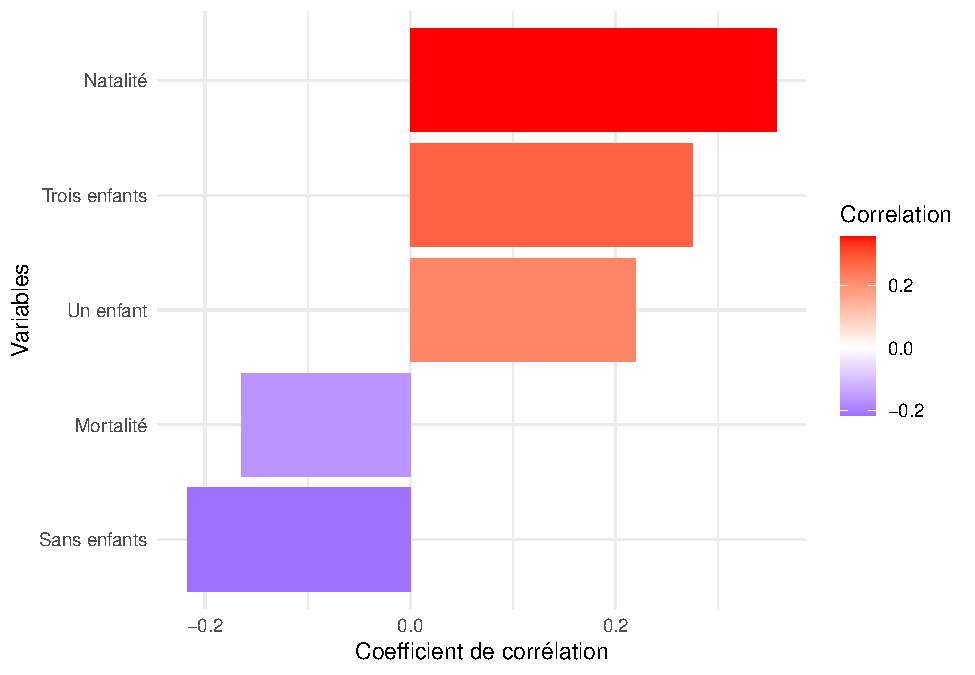
\includegraphics{Rapport_Projet_Stat_Ensai_files/figure-latex/unnamed-chunk-11-1.pdf}

\hypertarget{construction-de-la-matrice-de-poids}{%
\paragraph{Construction de la matrice de
poids}\label{construction-de-la-matrice-de-poids}}

Pour construire la matrice de poids, nous avons alors suivi ces étapes.
*

\begin{enumerate}
\def\labelenumi{\arabic{enumi}.}
\tightlist
\item
  Calculer les distances de Haversine entre chaque paire d'entités.
\item
  Définir un seuil de distance maximale (\(d_{max}\)) :

  \begin{itemize}
  \tightlist
  \item
    Si \(d_{ij} < d_{max}\), \(w_{ij} = \frac{1}{d_{ij}}\).
  \item
    Sinon, \(w_{ij} = 0\).
  \end{itemize}
\item
  Normaliser les poids pour que chaque ligne de la matrice ait une somme
  égale à 1 : \[
   w_{ij}^{norm} = \frac{w_{ij}}{\sum_{j} w_{ij}}.
  \]
\end{enumerate}

\begin{longtable}[]{@{}lr@{}}
\caption{Résultats du test de Moran}\tabularnewline
\toprule\noalign{}
& x \\
\midrule\noalign{}
\endfirsthead
\toprule\noalign{}
& x \\
\midrule\noalign{}
\endhead
\bottomrule\noalign{}
\endlastfoot
Moran I statistic & 0.1275832 \\
Expectation & -0.0003056 \\
Variance & 0.0000029 \\
\end{longtable}

Ainsi dans notre étude, nous avons trouvé un indice de Moran égale à
0.1275832. Le test nous a permi d'obtenir une p-value de 0. Ce qui
permet de conclure qu'il y a effectivement une autocorrélation positive
et significative entre les communes selon leur taux de consultations.

\hypertarget{discussion}{%
\section{Discussion}\label{discussion}}

\hypertarget{conclusion}{%
\section{Conclusion}\label{conclusion}}

\hypertarget{ruxe9fuxe9rences-bibliographiques}{%
\section{Références
bibliographiques}\label{ruxe9fuxe9rences-bibliographiques}}

\hypertarget{annexes}{%
\section{Annexes}\label{annexes}}

\begin{figure}
    \centering
    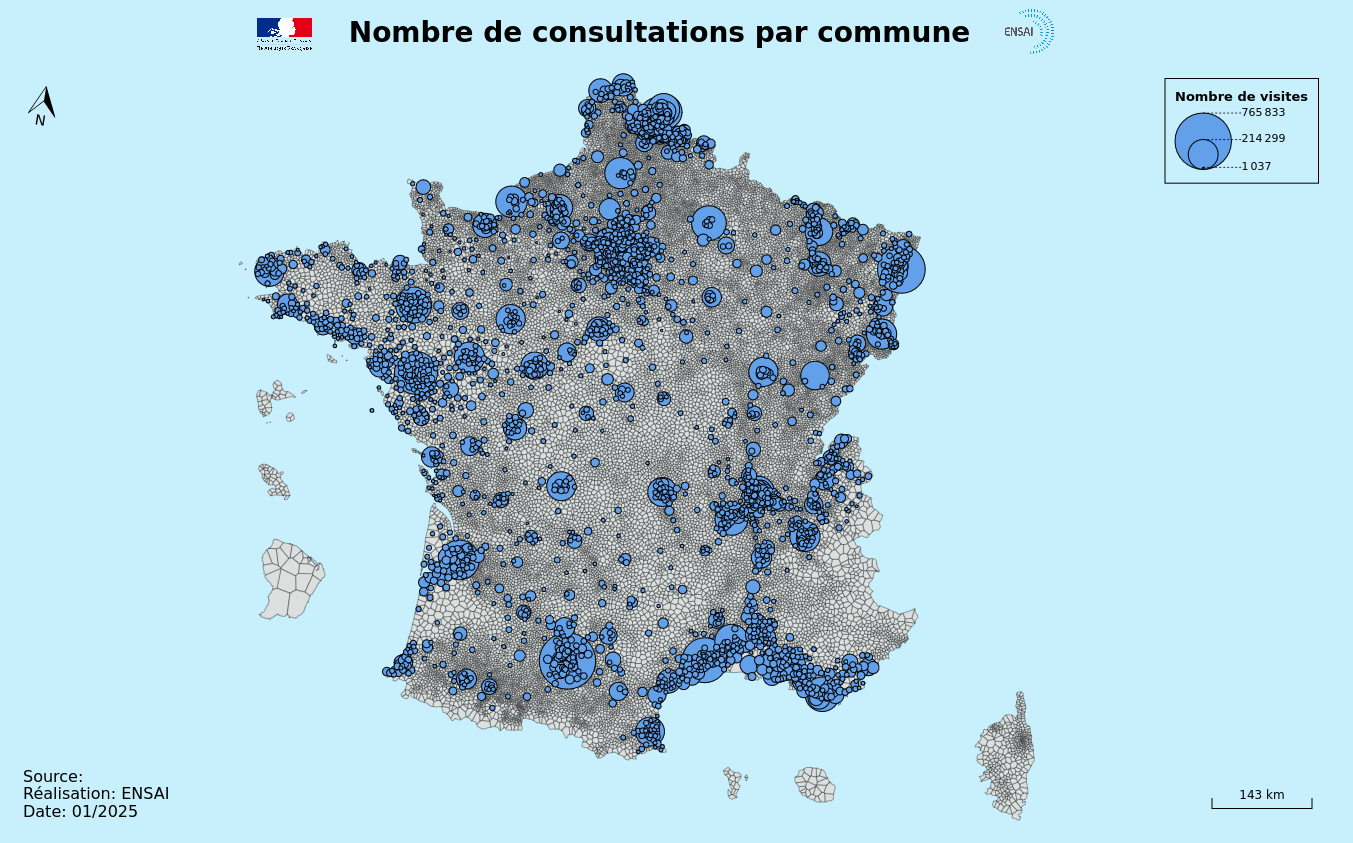
\includegraphics[width=1\linewidth]{../cartes/nombre_de_consulatations}
    \caption{Carte du nombre de consultations par commune}
    \label{fig:figure}
\end{figure}

\begin{figure}
    \centering
    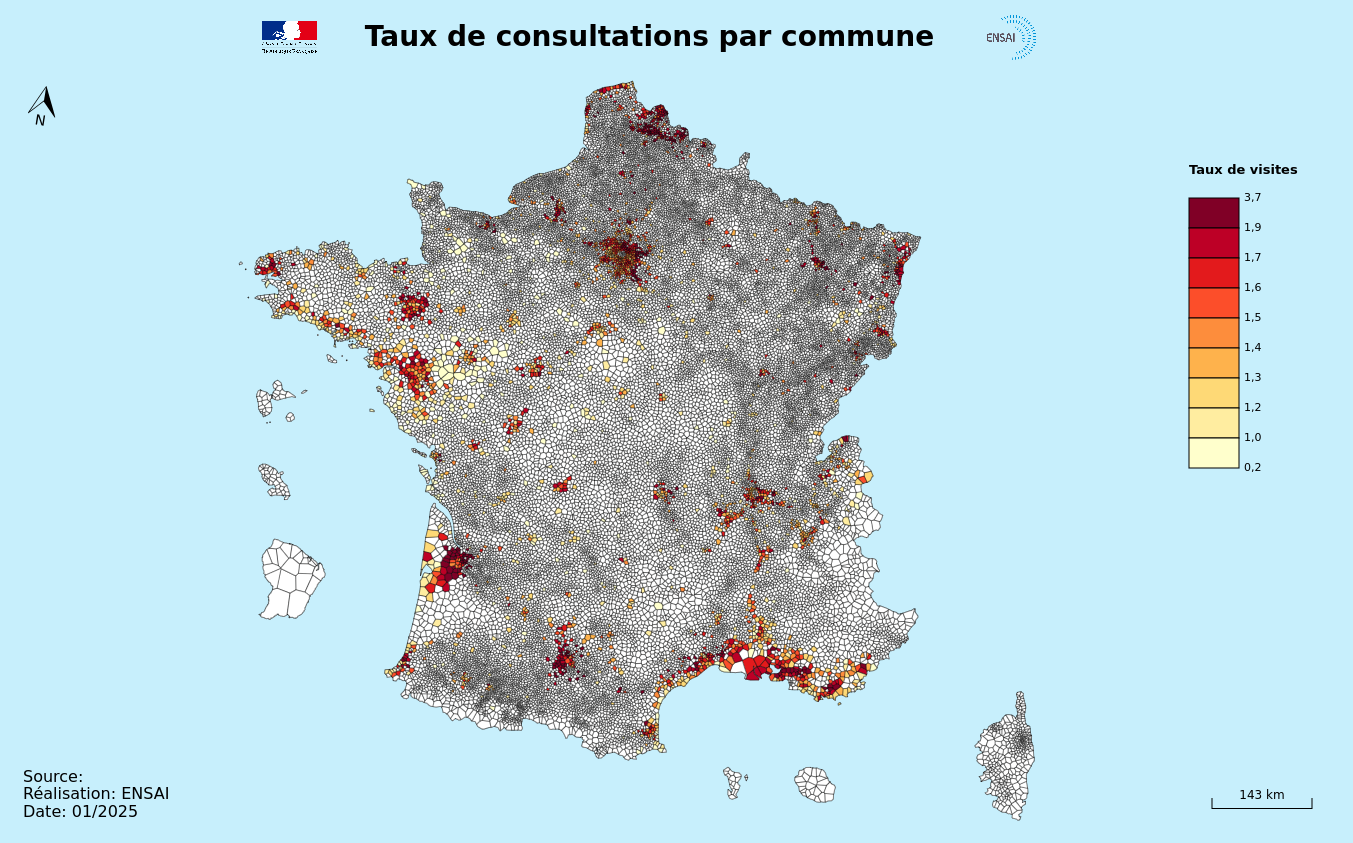
\includegraphics[width=1\linewidth]{../cartes/taux_de_consultations}
    \caption{Carte du taux de consultations par commune}
    \label{fig:figure}
\end{figure}

\begin{figure}
    \centering
    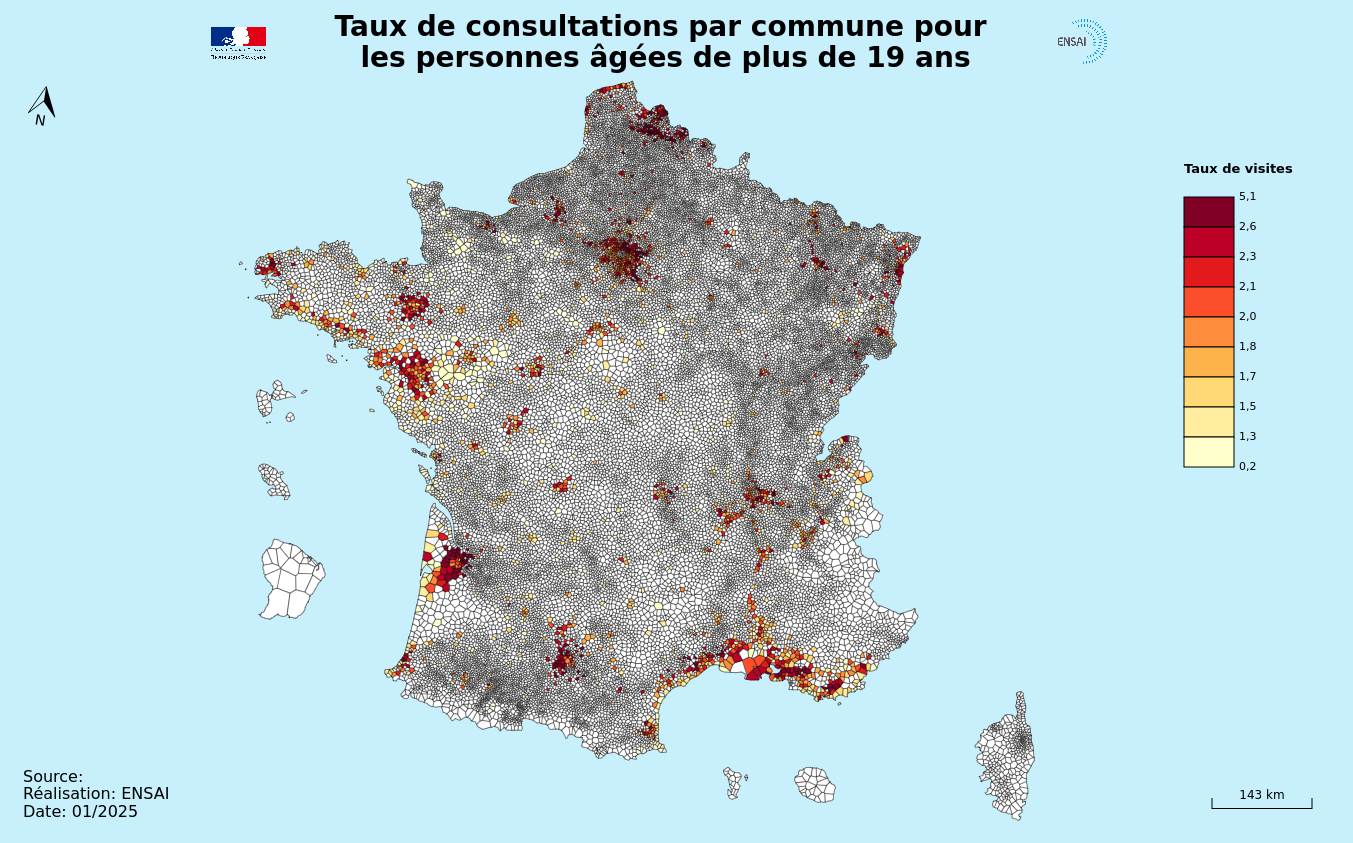
\includegraphics[width=1\linewidth]{../cartes/taux_de_consultations_plus_19_ans}
    \caption{Carte du taux de consultations par commune pour les plus de 19 ans}
    \label{fig:figure}
\end{figure}

\end{document}
